\documentclass[10pt]{article}
\usepackage{tikz}
\usetikzlibrary{arrows.meta, positioning, shapes}
\usepackage[margin=0.5in]{geometry}
\pagestyle{empty}

% Define colors matching the paper
\definecolor{colorSKVPP}{RGB}{70, 130, 180}
\definecolor{colorFreqSpec}{RGB}{220, 120, 50}
\definecolor{colorShadowKV}{RGB}{100, 160, 100}
\definecolor{colorStrict}{RGB}{180, 80, 80}
\definecolor{colorReactive}{RGB}{130, 90, 160}

\begin{document}

\begin{figure}[ht]
\centering
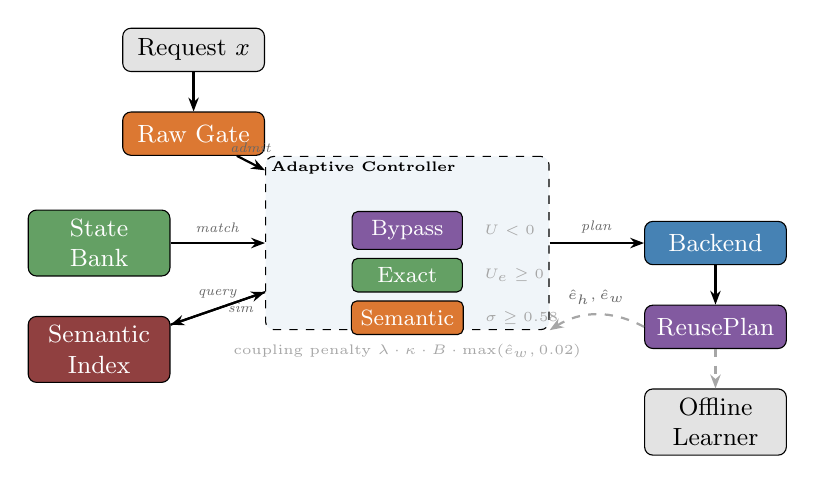
\begin{tikzpicture}[
  box/.style={draw,rounded corners=3pt,fill=#1,minimum width=1.8cm,
    minimum height=0.55cm,font=\small,align=center,text=white},
  box/.default=colorSKVPP,
  ibox/.style={draw,rounded corners=2pt,fill=#1,minimum width=1.4cm,
    minimum height=0.4cm,font=\footnotesize,align=center,text=white},
  gbox/.style={draw,rounded corners=3pt,fill=gray!22,minimum width=1.8cm,
    minimum height=0.55cm,font=\small,align=center},
  dbox/.style={draw,dashed,rounded corners=3pt,fill=#1!8,minimum width=3.6cm,
    minimum height=2.2cm,font=\small},
  arr/.style={-{Stealth[length=5pt]},thick},
  darr/.style={-{Stealth[length=5pt]},thick,dashed,gray!70},
  lbl/.style={font=\tiny,gray!80!black},
  node distance=0.5cm and 1.2cm,
]

% Input
\node[gbox] (req) {Request $x$};

% Raw gate
\node[box=colorFreqSpec, below=of req] (gate) {Raw Gate};

% Controller container
\node[dbox=colorSKVPP, below right=0cm and 0cm of gate] (ctrlbox) {};
\node[anchor=north west, font=\tiny\bfseries, inner sep=2pt] at (ctrlbox.north west) {Adaptive Controller};

% Controller subcomponents
\node[ibox=colorReactive, below=0.3cm of ctrlbox.north, yshift=-0.4cm] (bypass) {Bypass};
\node[ibox=colorShadowKV, below=0.1cm of bypass] (exact) {Exact};
\node[ibox=colorFreqSpec, below=0.1cm of exact] (semantic) {Semantic};

% Sub-labels inside controller
\node[font=\tiny, right=0.15cm of bypass, gray!70] {$U < 0$};
\node[font=\tiny, right=0.15cm of exact, gray!70] {$U_e \geq 0$};
\node[font=\tiny, right=0.15cm of semantic, gray!70] {$\sigma \geq 0.58$};

% State Bank
\node[box=colorShadowKV, left=of ctrlbox] (bank) {State\\Bank};

% Semantic Index
\node[box=colorStrict!80!black, below=of bank] (semidx) {Semantic\\Index};

% Backend
\node[box=colorSKVPP, right=of ctrlbox] (back) {Backend};

% ReusePlan
\node[box=colorReactive, below=of back] (plan) {ReusePlan};

% Offline Learner
\node[gbox, below=of plan] (learn) {Offline\\Learner};

% Coupling penalty note
\node[font=\tiny, gray!70, below=0.05cm of ctrlbox.south] {coupling penalty $\lambda \cdot \kappa \cdot B \cdot \max(\hat{e}_w, 0.02)$};

% Arrows
\draw[arr] (req) -- (gate);
\draw[arr] (gate) -- node[lbl,above]{\emph{admit}} (ctrlbox);

\draw[arr] (bank) -- node[lbl,above]{\emph{match}} (ctrlbox);
\draw[arr] (semidx) -- node[lbl,right]{\emph{sim}} (ctrlbox);
\draw[arr] (ctrlbox) -- node[lbl,above]{\emph{plan}} (back);

\draw[arr] (back) -- (plan);
\draw[darr] (plan) -- (learn);

% EWMA feedback loop
\draw[darr] (plan.west) to[bend right=30]
  node[pos=0.5,lbl,above]{\emph{$\hat{e}_h, \hat{e}_w$}} (ctrlbox.south east);

% Query semantic index
\draw[arr] (ctrlbox) -- node[lbl,above]{\emph{query}} (semidx);

\end{tikzpicture}
\caption{ShadowKV++ serving-time architecture. The Adaptive Controller branches into three admission paths: bypass (negative utility), exact reuse (bank match with $U_e \geq 0$), and semantic reuse (sketch similarity $\sigma \geq 0.58$ with utility gate). The coupling penalty $\lambda \cdot \kappa \cdot B \cdot \max(\hat{e}_w, 0.02)$ discounts semantic admits on high-$\kappa$ models. EWMA feedback ($\hat{e}_h, \hat{e}_w$) updates utility estimates after each request.}
\label{fig:architecture_v2}
\end{figure}

\end{document}
